\documentclass[main.tex]{subfiles}

\begin{document}
\chapter{Literature Review}
\chaplabel{literatureReview}
\section{Signal Processing}
%Implementation of autonomous detection and classification of subsurface objects, with a focus on identifying objects with a high likelihood of being a landmine. interpretation of the output signals from the GPR and metal detector will be processed with the aim to identify and confirm with a percentage the likelihood of a threat. Supplied data sets will be used to create and tune a detection algorithm to meet this goal, and operational trials will be conducted to test the effectiveness of the developed system.
% 
\subsection{Challenges in GPR signals}
\subsection{Challenges in MD signals}
\subsection{Chellanges in combination of GPR and MD signals}


\section{Navigation}
\subsection{Defining a Path Based on a Region}
\textbf{\color{red}{JONO CAN YOU TALK ABOUT DIFFERENT METHODS DO DEFINE A PATH BASED ON A REGION HERE, or maybe we dont even need to mention it, put in detailed design?}}

\subsection{Path Tracking}
\subsubsection{Geometric Path Tracking}
Geometric path tracking uses geometric relationships between a vehicle and a path to produce a control algorithm as a solution to the problem. Theories assume vehicles use the Ackermann method for steering so a simplified steering model can be used for the geometry. This reveals a relationship between the steering angle and the curvature that the non steering wheels will follow. Two of the most commonly used geometric vehicle models are Pure Pursuit and the Stanley Method \parencite{snider2009}.

Pure Pursuit uses a path 'look-ahead' distance to measure the future error between the vehicle and the path in real time which can then be steered to and corrected for. \Figref{purePursuitGeom} shows the geometry associated with Pure Pursuit at one point in time. It shows a goal point $(g_x, g_y)$ on the desired path at specified look-ahead distance $l_d$ in front of the vehicle. The steer angle is calculated based on an arc that would connect the centre of the non-steering axle to the goal point. When high curvatures are present in a path the controller may begin to cut corners due to a look-ahead distance that would effectively skip this portion of the path. Lateral error on a path of constant curvature may also be experienced due to geometric controller characteristics which do not take into account the curvature of a path. However, Pure Pursuit provides a very robust tracking algorithm when discontinuous curvatures are present \parencite{snider2009}. In general, for more accurate tracking a short look-ahead distance should be used but will eventually result in oscillation, for smoother tracking a long look-ahead distance should be used but this will reduce precision \parencite{snider2009}.
\begin{figure}[ht]
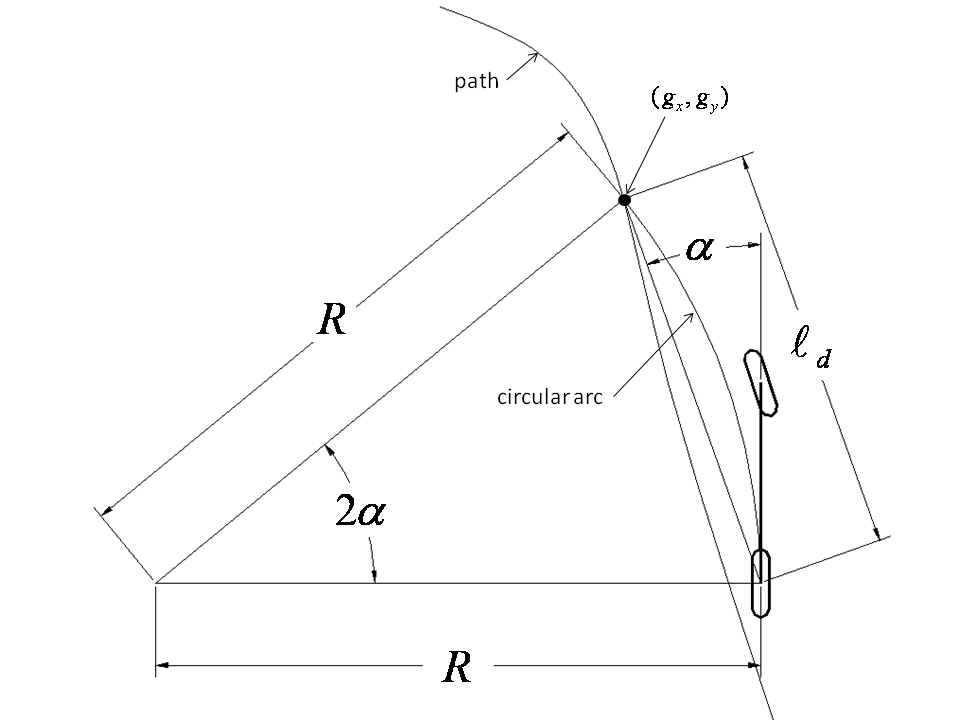
\includegraphics[width=0.6\textwidth]{3-LiteratureReview/purePursuitGoal.png}
\centering
\caption[Pure Pursuit Geometry]{Pure Pursuit Geometry \parencite{snider2009}} \figlabel{purePursuitGeom}
\end{figure}

The Stanley Model uses the lateral error between the centre of the wheels axle and the nearest path point  to determine steer angle (\figref{stanleyGeom}). It is simply set to the heading error which is given as the difference between the vehicles heading and the instantaneous heading of the nearest point on the path, $\theta_e$. An extra term is used when the lateral error is non zero which amplifies the steer angle to a new value of $\delta$.  This gives an effect so that as the error increases, or as the vehicle strays further from the path, the wheels are steered further towards the path in an attempt to correct. The Stanley Method is very well suited to higher speed tracking but can run into problems when curvature discontinuities are present in the path.
\begin{figure}[ht]
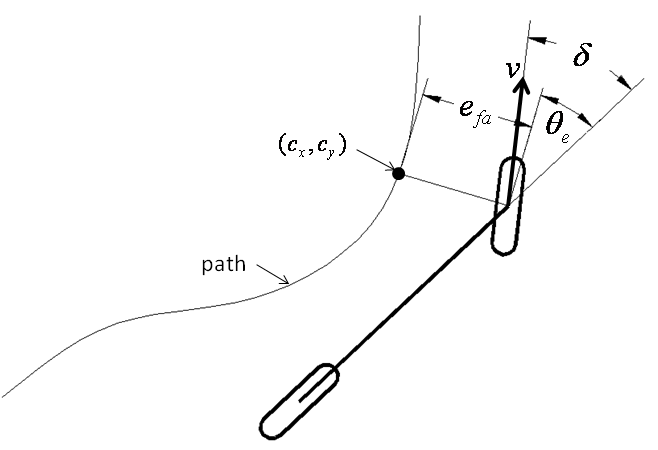
\includegraphics[width=0.5\textwidth]{3-LiteratureReview/stanleyMethod.png}
\centering
\caption[Stanley Method Geometry]{Stanley Method Geometry \parencite{snider2009}} \figlabel{stanleyGeom}
\end{figure}

Some limitations of geometric path tracking methods are related to the dynamics of a vehicle which are not present in the theory, namely the capabilities of a platform and its actuators. Due to this the method expects an instant response from elements such as the steering which is an issue when high path curvatures are present or when the curvature of the path suddenly changes. As a result the method cannot guarantee that the vehicle will follow a path as accurately as designed and at high speeds that vehicle may skid or tip \parencite{coulter1992}.

\subsubsection{Kinematic Path Tracking}
The kinematic model collapses a four wheeled vehicle into a two wheeled model, much like the geometric path tracking approach. The equations of motion for the simplified system are then used to relate the vehicle speed, change in heading error and change in lateral error to a user defined velocity and steer angle in path coordinates. In practice, the same trade off between performance and stability is apparent as in the geometric models, accurate tracking at low speeds but problems due to neglected dynamics at high speeds \parencite{snider2009}. This method is not as robust as Pure Pursuit and displays a similar behaviour to the Stanley Method when discontinuities in curvature are present.

\subsubsection{Dynamic Path Tracking}
A dynamic model approximates the real dynamics of a vehicle which was one of the downfalls of the previous examples. Similar to the kinematic model, the vehicle speed, heading error and lateral error are related to a user defined velocity and steer angle in path coordinates. Even though the dynamics of the vehicle are included in this model, extreme path dynamics can have as much of an effect on the efficiency of the path tracking \parencite{snider2009}. Discontinuities in the path still have a noticeable effect on accuracy and the steady state lateral error is still present. However, in a more realistic scenario a dynamic path tracking method does show overall improvement \parencite{snider2009}.

\subsection{Turning the Platform a Specified Angle}





\end{document}
